%\addcontentsline{toc}{chapter}{Development Process}
\chapter{Design}
On completion of my analysis and background planning for the project, I can now look at more detailed design for the application overview, and the individual component it comprises of. Becuase my application will present both a front-end GUI and back-end Javascript and WebGl, I will split my design into two sections. The reasoning for this is becuase I would prefer to have the GUI and logic of the application to be decoupled, so that the code can be changed in the Javascript easily without having to affect the user interface. Other than planning the application itself, it is also important I plan what key assisting services I use, such as how I intend on versioning my code, to how I will deploy my code.

\section{Overall Architecture}
As a summary of the architecture of my planned application, the best way to design in more detail is to lay out a primary design pattern. For the purpose of an application which will allow for user interaction, which will be processed by code in the back-end, I have decided to go ahead with a Model-view-controller approach. Using the MVC pattern means I can separate the GUI from the logic code as I wanted to, and have the GUI exists without knowledge of the back-end. This is also the same with the model, where the primary code for calculating manoeuvre movements and animations should be possible without knowledge of the view, but instead use the controller as a intermediary. See figure ~\ref{fig:mvc} for the MVC pattern I plan to use. 

\begin{figure}[h!]
  \centering
      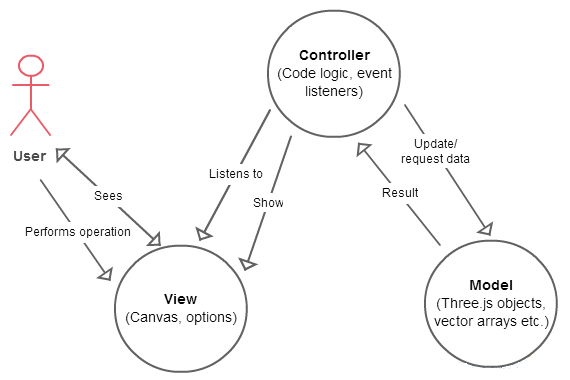
\includegraphics[width=0.8\textwidth]{images/mvc.png}
  \caption{Model View Controller diagram for my proposed application. Shows the planned interactions between different subjects within my application.}
  \label{fig:mvc}
\end{figure}

Because I have already chosen three.js as library of choice for creating any graphics and physics objects, these will already form my model or models. Each manoeuvre for instance will be reflected as a set of vectors which will form the shapes of the Aresti flight paths, and should be accessible and changeable through the controller to the view(in this case the canvas in my GUI).

The controller will be the most crucial part I implement, as it will need to be able to communicate with the three.js objects, the canvas disaplaying the animation, and detect controls from the user. For this piece of the pattern, I will enforce some other design patterns to 

Finally, the view will be represented as the canvas and controls on the web page. Since on both the canvas and the options menu can have an affect on the model, the controller will listen for changes on either, and then call the relevent operations to affect the model, and again reflect this back onto the view. The view will not know anything of the controller nor the model, so adding any new options or displayable information will be easier and not conflict with any current elements.

\section{Back-end logic and design}
The first of the two design categories concentrates on the JavaScript that will act as the functions to run each of the proposed features of the application. The code on this side will be responsible for maintaining contact with the GUI, and more importantly the WebGL canvas on the web page. To make the code be as maintainable and run effectively as possible, I will look into a variety of design patterns.

\subsection{Design patterns}
Because I am using a hybrid of waterfall and FDD at this stage of the project, using a changing range of design patterns for my JavaScript and GUI architecture is possible. Through the implimentation stage of this report, some of these may patterns mentioned may not be used anymore and replaced for different ones depending on changing requirements and progress. Using the implement, refactor and test iteration approach should allow for this.

Starting by looking at 
%Talk about rejected design patterns

\subsection{Module diagram}
Because much of the code I will be implementing will hold various Three.Js objects, I have decided that modulating methods and objects will be better than simulating classes seeing as JavaScript is a class-less language. This is a pattern known as the module pattern. Although this may appear less object orientated, modules allow for more robust archetecture where units of code can be separated and organised. Modules are slightly similar to classes in the way they can hide code that should not be accessable to other modules by encapsulates privacy. When code is modulated, and then that module is called upon by another, only a public API is returned, and other methods in that module are kept private from being used in other parts of the application. These private methods are good for use as supporting methods, holding such things as calculations, or private variables for getters and setters. Again, this is a similar case to the traditional class diagram.

There are currently a selection of libraries that allow for modules in JavaScript. The most promininent, and the one I would like to use is called RequireJS, which promises the increase in speed and quality of code. RequireJS works by dynamically loading JavaScript files on the fly, where the code has from the other module is usable once loaded into the module calling it. Once modules are loaded into an object form in whatever the developer needs to name it, its public variables and methods can then be accessed. See figure ~\ref{fig:module} on how modules are used. In my case, modules would be useful in enforcing the MVC pattern in the way that it 

\lstset{language=JavaScript}
\medskip
\begin{lstlisting}[caption=Example showing how RequireJS loads in another module or Javascript file which in this case is loading up the util javascript module and naming it as object 'util' for use in the code]
require(["helper/util"], function(util) { 
	
	function private_function(){
		// only accessable from in this module
	}
	return {
		public_function: function(){
			// can be called if this module is loaded into another module
		}
	}
}
\end{lstlisting}
\label{fig:module}


In order to create a basis for modulating code, I should first look to seperate the features I listed in the analysis section of this report into categories. These categories will then help me to determine how I could structure my application in as best object orientated way as possible.

The categories I have been able to come to are:
\begin{itemize}
  \item Main- initiating other modules, beginning the application.
  \item Animation- Playing, and controlling speed, physics of animation.
  \item Loading manoeuvres at start of application.
  \item Saving and loading animations
  \item Cameras- Creating and controlling cameras movements
  \item GUI controlling- control and edit GUI controls, and appearence from back-end. Also including the possible movie reel live animatiion.
  \item Canvas controls- Allowing the user to move along the canvas, and zoom.
\end{itemize}

Now I have a stable list of categoried features, I am able to create a diagram to represent what modulated layout my applicatioon will use. Becuase of the way modules handle public and private variables, have public and have private methods, means that this is very reminiscent of a standard class diagram.

\begin{figure}[h!]
  \centering
      %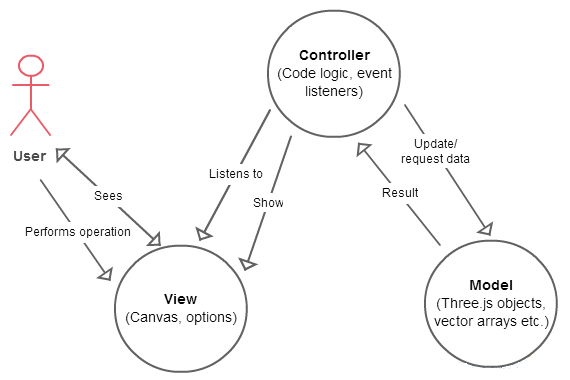
\includegraphics[width=0.8\textwidth]{images/mvc.png}
  \caption{Module diagram displaying the various communications between modules, and how they are connected to the GUI in the MVC way.}
  \label{fig:mvc}
\end{figure}

The module diagram shows a number of things...

\subsection{Object and storage formatting}

\subsection{Naming conventions}

\section{User Interface}

\subsection{GUI Use-case}

\subsection{CSS and wireframe design}

\section{Planned use of services}

% word count -252 = 181
%You should concentrate on the more important aspects of the design. It is essential that an overview is presented before going into detail. As well as describing the design adopted it must also explain what other designs were considered and why they were rejected.The design should describe what you expected to do, and might also explain areas that you had to revise after some investigation.Typically, for an object-oriented design, the discussion will focus on the choice of objects and classes and the allocation of methods to classes. The use made of reusable components should be described and their source referenced. Particularly important decisions concerning data structures usually affect the architecture of a system and so should be described here.How much material you include on detailed design and implementation will depend very much on the nature of the project. It should not be padded out. Think about the significant aspects of your system. For example, describe the design of the user interface if it is a critical aspect of your system, or provide detail about methods and data structures that are not trivial. Do not spend time on long lists of trivial items and repetitive descriptions. If in doubt about what is appropriate, speak to your supervisor. You should also identify any support tools that you used. You should discuss your choice of implementation tools - programming language, compilers, database management system, program development environment, etc.Some example sub-sections may be as follows, but the specific sections are for you to define.
